% Definition of the General Document Format
\documentclass[a4paper,12pt,headsepline]{scrartcl}

% Use Umlauts with UTF8
\usepackage[utf8]{inputenc}

% Variables
%Variables that should be available throughout the entire document
\newcommand{\subjectDocument}{THESIS TOPIC TITLE}
\newcommand{\titleDocument}{Master Thesis}
\newcommand{\affiliationDocument}{Fachhochschule Dortmund \\ Department of Computer Science \\ Master's Program \\ Master thesis}
\newcommand{\degreeDocument}{for the attainment of the academic degree\\ Master of Engineering}


% additional packages
% Include graphics from PNG files
\usepackage{graphicx}

% Use German special characters and hyphenation
\usepackage[english]{babel}

% Include Euro symbol
\usepackage[right]{eurosym}

% Character encoding
\usepackage[T1]{fontenc}

\usepackage{lmodern}

% Enable floating images
%\usepackage{floatflt}

% Enable multi-page tables
\usepackage{longtable}

% Support for fonts
%\newcommand{\changefont}[3]{ 
%\fontfamily{#1} \fontseries{#2} \fontshape{#3} \selectfont}

% Package for page margins and setting margins
\usepackage{geometry}
\geometry{left=3.5cm, right=2cm, top=2.5cm, bottom=2cm}

% Package for boxes in text
\usepackage{fancybox}

% Breaks long URLs "nicely"
\usepackage[hyphens,obeyspaces,spaces]{url}

% Package for text colors
\usepackage{color}

% Import mathematical symbols
\usepackage{amssymb}
\usepackage{wasysym}

% Header on every page (old, centered)
%\pagestyle{headings}
\usepackage{xhfill}

% Generates table of contents with cross-references to sections (PDF version)
\usepackage[bookmarksnumbered,pdftitle={\titleDocument},hyperfootnotes=false]{hyperref}
%\hypersetup{colorlinks, citecolor=red, linkcolor=blue, urlcolor=black}
%\hypersetup{colorlinks, citecolor=black, linkcolor= black, urlcolor=black}
% new headers with fancy package
\usepackage{fancyhdr} % Load package
\pagestyle{fancy} % Own page style
\fancyhf{} % Clear all header and footer fields
\fancyhead[L]{\nouppercase{\leftmark}} % Left header
\fancyhead[C]{} % Centered header
\fancyhead[R]{\thepage} % Right header
\renewcommand{\headrulewidth}{0.4pt} % Upper separator line
%\fancyfoot[C]{\thepage} % Page number
%\renewcommand{\footrulewidth}{0.4pt} % Lower separator line

% for tables
\usepackage{array}

% Round brackets for citations
%\usepackage[numbers,round]{natbib}

% Citation style - Harvard method: Author abbreviation + Year
\bibliographystyle{alphadin}

% Disables the extra space that LaTeX usually inserts after a period.
%\frenchspacing

% Package for line spacing
\usepackage{setspace}

% for figure captions
\usepackage{capt-of}

% for index
\usepackage{makeidx}

% Configure the table of contents
\usepackage{tocbasic}
\DeclareTOCStyleEntries[
  raggedentrytext,
  numwidth=0pt,
  numsep=1ex,
  dynnumwidth,
]{tocline}{chapter,section,subsection,subsubsection,paragraph,subparagraph}
\DeclareTOCStyleEntries[
  indent=0pt,
  linefill=\TOCLineLeaderFill,
]{tocline}{section,subsection,subsubsection,paragraph,subparagraph}


% for listings
\usepackage{listings}
\lstset{numbers=left, numberstyle=\tiny, numbersep=5pt, keywordstyle=\color{black}\bfseries, stringstyle=\ttfamily,showstringspaces=false,basicstyle=\footnotesize,captionpos=b}
\lstset{language=java}

% Create index
\makeindex

% Abbreviations
\usepackage[english]{nomencl}
\let\abbrev\nomenclature

% Abbreviations LiveTex Version
% Title of the abbreviations list
\renewcommand{\nomname}{Abbreviations}
% Distance between abbreviation and explanation
\setlength{\nomlabelwidth}{.25\textwidth}
% Space between abbreviation and explanation with dots
\renewcommand{\nomlabel}[1]{#1 \dotfill}
% Variation of the distance between the individual abbreviations
\setlength{\nomitemsep}{-\parsep}
% Create index with abbreviations
\makenomenclature
%\makeglossary

% Abbreviations TeTEX Version
% \usepackage[german]{nomencl}
% \makenomenclature
% %\makeglossary
% \renewcommand{\nomname}{Abbreviations}
% \AtBeginDocument{\setlength{\nomlabelwidth}{.25\columnwidth}}
% \renewcommand{\nomlabel}[1]{#1 \dotfill}
% \setlength{\nomitemsep}{-\parsep}

% Optional: Prevent single lines at the beginning of a page (orphans)
% \clubpenalty = 10000
% Optional: Prevent single lines at the end of a page (widows)
% \widowpenalty = 10000
% \displaywidowpenalty = 10000

\begin{document}
% include hyphenation suggestions here
% Here you need to include all the words that LaTeX does not hyphenate correctly on its own or for which you want to specify the exact hyphenation
\hyphenation{
Film-pro-duc-ers
Lux-em-bourg
Soft-ware-com-po-nent
time-in-ten-sive
}


% Use Helvetica font
%\usepackage{helvet}
%\renewcommand\familydefault{\sfdefault}

% Blank page at the beginning
%\thispagestyle{empty} % creates a page without header / footer
%\mbox{}
%\newpage

% Title page %
\thispagestyle{empty}

%\end{verbatim}
\begin{center}
\doublespacing
\textbf{\LARGE{\subjectDocument}}\\
\singlespacing
\begin{verbatim}


\end{verbatim}
{\large\affiliationDocument}
\begin{verbatim}

\end{verbatim}
{\large\degreeDocument}
\end{center}
\begin{verbatim}




\end{verbatim}
\begin{center}
{\large{by Student Name \\ born on 1/01/2024}}
\end{center}
\begin{verbatim}







\end{verbatim}
\begin{flushleft}
\begin{tabular}{llll}
\textbf{Matriculation Number :} & & NXXXXXXXX & \\
\textbf{Supervisor   :} & & Prof. XXXXXXXXXXX &\\
\end{tabular}
\begin{verbatim}



  
\end{verbatim}
\begin{tabular}{l}
Place, DD.MM.2024
\end{tabular}
\end{flushleft}


% Roman numeration
\pagenumbering{roman}

% 1.5 line spacing
\onehalfspacing

\newpage

% Introduction / Abstract
\thispagestyle{empty}
\section*{Abstract}



% Single line spacing
\singlespacing

\newpage
% Start page numbering at table of contents
\setcounter{page}{1}

% Display table of contents
\thispagestyle{empty}
\tableofcontents

\newpage
% the list of figures
% Version 1: Display list of figures WITH leading numbering
\listoffigures
% List of figures should appear in the table of contents
\addcontentsline{toc}{section}{List of Figures}

% Version 2: Display list of figures WITHOUT leading numbering
%\begingroup
%\renewcommand\numberline[1]{}
%\listoffigures
%\endgroup


% the list of tables
\newpage
% \fancyhead[L]{List of Figures / Abbreviations} % Left header
% Display list of tables
\listoftables
% List of tables should appear in the table of contents
\addcontentsline{toc}{section}{List of Tables}

%% WORKAROUND for Listings
%\makeatletter% --> De-TeX-FAQ
%\renewcommand*{\lstlistoflistings}{%
%  \begingroup
%    \if@twocolumn
%      \@restonecoltrue\onecolumn
%    \else
%      \@restonecolfalse
%    \fi
%    \lol@heading
%    \setlength{\parskip}{\z@}%
%    \setlength{\parindent}{\z@}%
%    \setlength{\parfillskip}{\z@ \@plus 1fil}%
%    \@starttoc{lol}%
%    \if@restonecol\twocolumn\fi
%  \endgroup
%}
%\makeatother% --> \makeatletter
% the list of listings
\newpage
\fancyhead[L]{List of Listings} % Left header
\renewcommand{\lstlistlistingname}{List of Listings}
\lstlistoflistings
% List of listings should appear in the table of contents
\addcontentsline{toc}{section}{List of Listings}
%%%%

% the list of abbreviations
\newpage
% display the list of abbreviations
\fancyhead[L]{Abbreviations} % Left header
\nomenclature{UGC}{User Generated Content}
\nomenclature{CSS}{Cascading Style Sheets}
\nomenclature{JS}{JavaScript}
\nomenclature{SQL}{Structured Query Language}
\nomenclature{GPL}{GNU General Public License}
\nomenclature{GNU}{GNU is not Unix}
\nomenclature{LGPL}{GNU Lesser General Public License}
\nomenclature{XMPP}{Extensible Messaging and Presence Protocol}
\nomenclature{IM}{Instant Message}
\nomenclature{CMS}{Content Management System}
\nomenclature{RSS}{Really Simple Syndication}
\nomenclature{JSON}{JavaScript Object Notation}
\nomenclature{HTML}{Hypertext Markup Language}
\nomenclature{TDD}{Test-driven development}
\nomenclature{GUI}{Graphical User Interface}
\nomenclature{KPI}{Key Performance Indicator}
\nomenclature{WWW}{World Wide Web}
\nomenclature{OCR}{Optical Character Recognition}
\nomenclature{ERM}{Entity Relationship Modell}

\printnomenclature[3cm]
% List of abbreviations should appear in the table of contents
\addcontentsline{toc}{section}{List of Abbreviations}


%%%%%%% INTRODUCTION %%%%%%%%%%%%
\newpage
\fancyhead[L]{\nouppercase{\leftmark}} % Left header

% 1.5 line spacing
\onehalfspacing

% Arabic page numbering from here
\pagenumbering{arabic}

% Alternative inclusion of the abstract in chapter "0" if desired
%\setcounter{section}{-1}
%\setcounter{page}{0}

% Option: inclusion of abstract
%\section*{Abstract}


%\newpage

% individual chapters are included here
\section{Introduction}\label{Introduction}

The autonomous industry has seen instantaneous growth, and the positioning of vehicles serves as a
critical milestone for a wide range of applications, ranging from advanced driver-assistance systems
(ADAS) to autonomous driving. A vehicle should realize its position concerning the environment at
level 3 or above for autonomous driving, according to the Society of Automotive Engineers, where
at level 0, the driver has full control of the vehicle, and at level 5, the vehicle has full control for all
challenging environments [14]. Germany became the first to embrace Level 3 automated driving
technology, which signifies a significant step towards autonomous driving. With major
manufacturers like BMW and Mercedes offering Level 3 systems in the European market and Level
4 testing in progress, the automotive industry is rapidly advancing towards fully autonomous vehicles
[15]. The shift towards higher levels of automation not only improves the safety and efficiency of
the vehicle but also paves the way for a future where self-driving cars are the norm.

Additionally, artificial intelligence and sensor technology advancements are key components in
developing reliable autonomous navigation systems. These systems must be able to interpret and
respond to complex environments in real-time to ensure safe and efficient operation. Perception,
localization and mapping, path planning, and control are the four main components of autonomous
driving. With more ADAS systems coming into the picture, more AD functions are added to the
latest mass-production vehicle, requiring immense testing and verification. This process needs
ground truth data like vehicle position, velocity, number of objects, and more to play an important
role in defining the accuracy of these systems.

A few major challenges faced by the automotive industry.
1. Accuracy: Achieving this level of precision is essential, especially for applications like
autonomous driving and advanced navigation systems.
2. Positioning Under Bridges: GNSS signals can be weak or blocked under bridges,
necessitating reliance on IMU data and dead reckoning.
3. Positioning in Tunnels: Similar to under bridges, GNSS signals are typically unavailable in
tunnels. Accurate dead reckoning is crucial here.
4. Positioning in GNSS-Denied Environments for Extended Periods: Maintaining accuracy
over time without GNSS support is challenging due to the potential drift in IMU data.
5. Ground Truth for Motion Planning: Accurate positioning data is critical for lane detection
and lane-keeping systems in autonomous vehicles.
6. Reference Point for Localization Algorithms: High accuracy in vehicle localization is
necessary for safe and efficient navigation.
7. Vehicle Location in Complex Interchanges: Identifying precise vehicle location in complex
highway interchanges like stack or cloverleaf intersections, where multiple layers and
directions can confuse navigation systems.
\newpage

\section{Chapter 2}\label{main section}

Text of the first section... Lorem ipsum dolor sit amet, consetetur sadipscing elitr, sed diam nonumy eirmod tempor invidunt ut labore et dolore magna aliquyam erat, sed diam voluptua. At vero eos et accusam et justo duo dolores et ea rebum. Stet clita kasd gubergren, no sea takimata sanctus est Lorem ipsum dolor sit amet. Lorem ipsum dolor sit amet, consetetur sadipscing elitr, sed diam nonumy eirmod tempor invidunt ut labore et dolore magna aliquyam erat, sed diam voluptua. At vero eos et accusam et justo duo dolores et ea rebum. Stet clita kasd gubergren, no sea takimata sanctus est Lorem ipsum dolor sit amet.

\subsection{Subsection 1}\label{unterabschnitt_1}

First Subsection

\subsection{Subsection 2}\label{unterabschnitt_2}

Second Subsection

\subsection{Subsection 3}\label{unterabschnitt_3}

Third Subsection

\newpage

\section{Chapter 3}\label{main_section_2}

% Example of an image with a footnote
\begin{figure}[htb]
    \centering
    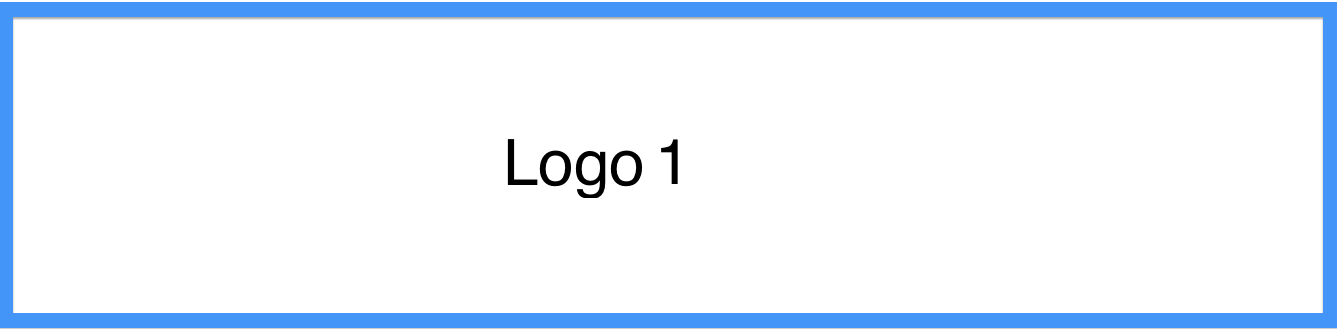
\includegraphics[width=0.4\textwidth,angle=45]{abb/logo1}
    \caption[Example of a figure description]{Example of a figure description\footnotemark}
    \label{fig:example1}
\end{figure}
\footnotetext{Image source: Example of an image source}

% Example of image integration
\begin{figure}[htb]
    \centering
    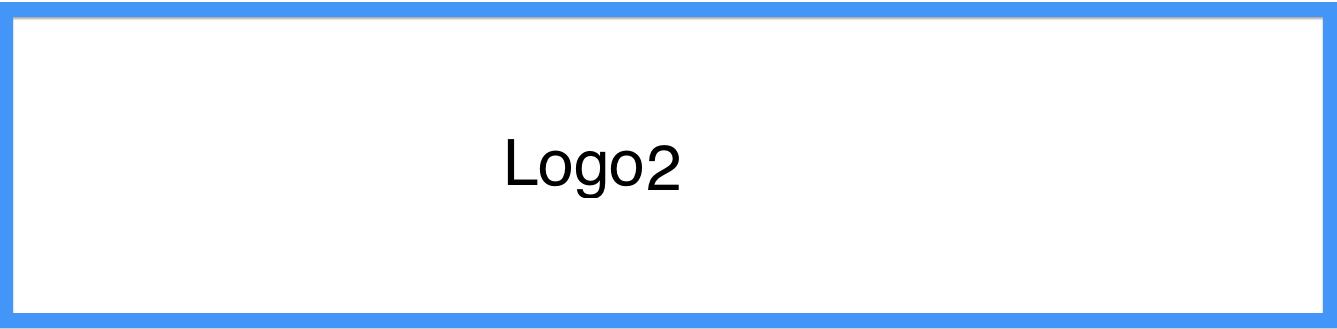
\includegraphics[width=0.3\textwidth,angle=0]{abb/logo2}
    \caption[Description]{Description \cite[p. 96]{mf2005}}
    \label{fig:description}
\end{figure}

% Example: Reference to figure
Figure~\ref{fig:description} [p.\pageref{fig:description}]

% Example: Table 
\begin{table}[!h]
    \begin{center}
        \begin{tabular}{ | l | c | }
            \hline
            Heading 1 & Heading 2 \\ \hline \hline
            Info 1 & Info 2 \\ \hline
            Info 3 & Info 4 \\ \hline
            \hline
            \multicolumn{2}{|c|}{Info in one cell} \\
            \hline
        \end{tabular}
        \caption[Description of the table]{Description of the table \cite[p. 13]{mm2009}}
    \end{center}
\end{table}


% Example for source code listings
\lstset{language=xml}
\begin{lstlisting}[frame=htrbl, caption={The file {\normalfont \ttfamily  data-config.xml} serves as an example for XML source code}, label={lst:dataconfigxml}]
    <dataConfig>
    <dataSource type="JdbcDataSource" 
    driver="com.mysql.jdbc.Driver"
    url="jdbc:mysql://localhost/bms_db"
    user="root" 
    password=""/>
    <document>
    <entity name="id"
    query="select id, htmlBody, sentDate, sentFrom, subject, textBody
    from mail">
    <field column="id" name="id"/>
    <field column="htmlBody" name="text"/>
    <field column="sentDate" name="sentDate"/>
    <field column="sentFrom" name="sentFrom"/>
    <field column="subject" name="subject"/>
    <field column="textBody" name="text"/>
    </entity>
    </document>
    </dataConfig>
\end{lstlisting}

\lstset{language=java}
\begin{lstlisting}[frame=htrbl, caption={This listing shows Java source code}, label={lst:result2}]
    /* generate TagCloud */
    Cloud cloud = new Cloud();
    cloud.setMaxWeight(_maxSizeOfText);
    cloud.setMinWeight(_minSizeOfText);
    cloud.setTagCase(Case.LOWER);
    
    /* evaluate context and find additional stopwords */
    String query = getContextQuery(_context);
    List<String> contextStoplist = new ArrayList<String>();
    contextStoplist = getStopwordsFromDB(query);
    
    /* append context stoplist */
    while(contextStoplist != null && !contextStoplist.isEmpty())
    _stoplist.add(contextStoplist.remove(0));
    
    /* add cloud filters */
    if (_stoplist != null) {
        DictionaryFilter df = new DictionaryFilter(_stoplist);
        cloud.addInputFilter(df);
    }
    /* remove empty tags */
    NonNullFilter<Tag> nnf = new NonNullFilter<Tag>();
    cloud.addInputFilter(nnf);
    
    /* set minimum tag length */
    MinLengthFilter mlf = new MinLengthFilter(_minTagLength);
    cloud.addInputFilter(mlf);
    
    /* add taglist to tagcloud */
    cloud.addText(_taglist);
    
    /* set number of shown tags */	    
    cloud.setMaxTagsToDisplay(_tagsToDisplay);
\end{lstlisting}


% Example for formulas
The assignment of all possible values that a random variable can take is called the \emph{distribution function} of $X$.

\begin{quotation}
    The function F: $\mathbb{R} \rightarrow$ [0,1] with $F(t) = P (X \le t)$ is called the distribution function of $X$ \cite[pp. 42--49]{mm2009}.
\end{quotation}

\begin{quotation}
    For a continuous random variable $X: \Omega \rightarrow \mathbb{R}$, an integrable, non-negative real function $w: \mathbb{R} \rightarrow \mathbb{R}$ with $F(x) = P(X \le x) = \int_{-\infty}^{x} w(t)dt$ is called the \emph{density} or \emph{probability density} of the random variable $X$.\footnote{Mustermann, see~\cite{mf2005}~[p.56]}
\end{quotation}

\newpage

% further chapters can be created and entered here
% ....

\section{Conclusion}\label{conclusion}

\subsection{Summary and Conclusion}

\subsection{Outlook}

\newpage



% Single line spacing
\singlespacing
% Bibliography should appear in the table of contents
\newpage
\phantomsection
\addcontentsline{toc}{section}{Bibliography}
% Display bibliography
\renewcommand\refname{Bibliography}
\bibliography{Hauptdatei}

%% Index should be called Keyword Index
% \newpage
% % Keyword index should appear in the table of contents
% \addcontentsline{toc}{section}{Keyword Index}
% \renewcommand{\indexname}{Keyword Index}
% % Display keyword index
% \printindex

\onehalfspacing
% possibly appendix
\newpage
\phantomsection
\addcontentsline{toc}{section}{Appendix}
\fancyhead[L]{Appendix} % Left header
\subsection*{Appendix}\label{appendix}

The appendix consisting of images and texts...

% Example of image integration
\begin{figure}[htb]
 \centering
 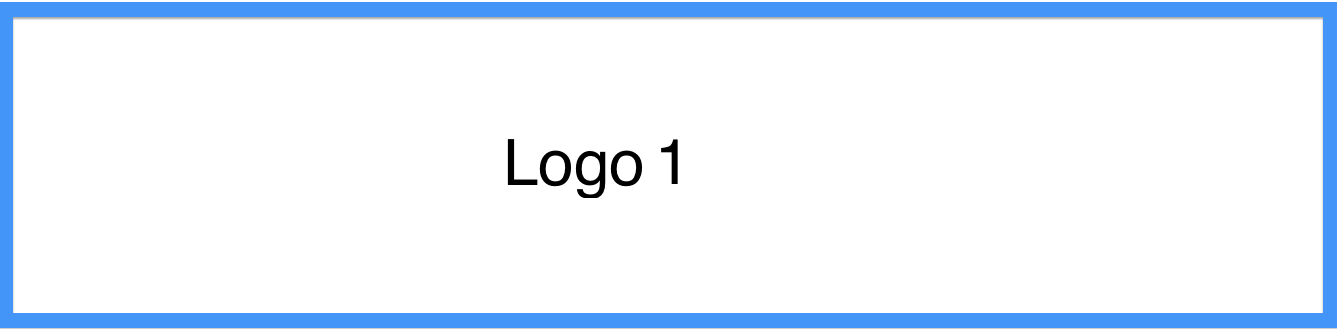
\includegraphics[width=0.3\textwidth,angle=0]{abb/logo1}
 \caption[Figure in the Appendix]{Figure in the Appendix}
 \label{fig:figure_in_appendix}
\end{figure}

Lorem ipsum dolor sit amet, consetetur sadipscing elitr, sed diam nonumy eirmod tempor invidunt ut labore et dolore magna aliquyam erat, sed diam voluptua. At vero eos et accusam et justo duo dolores et ea rebum. Stet clita kasd gubergren, no sea takimata sanctus est Lorem ipsum dolor sit amet. Lorem ipsum dolor sit amet, consetetur sadipscing elitr, sed diam nonumy eirmod tempor invidunt ut labore et dolore magna aliquyam erat, sed diam voluptua. At vero eos et accusam et justo duo dolores et ea rebum. Stet clita kasd gubergren, no sea takimata sanctus est Lorem ipsum dolor sit amet.
 
\newpage
\thispagestyle{empty}
\subsection*{Declaration of Authorship}\label{eigenstaendigkeit}

{\small 
I hereby declare that I have produced the present work independently and without any unauthorized assistance and have used only the sources and aids indicated. All passages that are taken literally or in spirit from published or unpublished writings and other sources are marked as such. This work has not been presented to any examination authority in the same or a similar form. \\ \\

{
\setlength{\parindent}{0pt}
\begin{tabular}{@{}lr@{}}
\textbf{\large Declaration of Used Tools} & \\ \\
Correction service of the university or department used: & Yes \Square~No \Square \\ \\
Use of an external (commercial) correction service: & Yes \Square~No \Square \\ 
if yes, which one \hrulefill &  \\ \\
The following persons additionally proofread the work: & \\
\hrulefill & \\
\hrulefill & \\ \\
Use of language models for text creation (e.g. ChatGPT), & Yes \Square~No \Square \\
if yes, which ones and in which sections: & \\
\hrulefill & \\ \\
Translation tools (e.g. Google Translator, DeepL), & Yes \Square~No \Square \\
if yes, which ones and in which sections: & \\
\hrulefill & \\ \\
Use of software for language correction (e.g. Grammarly), & Yes \Square~No \Square \\
if yes, which ones and in which sections: & \\
\hrulefill & \\ \\
Use of other aids: & \\
\hrulefill & 
\end{tabular}} \\ \\ \\
\setlength{\parindent}{0pt}
I acknowledge that my thesis may be checked using plagiarism detection software. \\ \\
I confirm that the above statements have been completed fully and to the best of my knowledge. \\ 

\rule{8cm}{1pt} \\
Date, Author's Signature}

\end{document}